% !TeX program = pdflatex
\documentclass[11pt,a4paper]{article}

\usepackage[margin=2.5cm]{geometry}
\usepackage{amsmath,amssymb}
\usepackage{booktabs}
\usepackage{graphicx}
\graphicspath{{figs/}}
\usepackage{xcolor}
\usepackage[colorlinks=true,allcolors=blue!60!black]{hyperref}
\usepackage{microtype}

% \belowcaptionskip defaults to 0pt, so a caption placed above a table sits
% flush against its top rule. Load after hyperref, as the package requires.
\usepackage[skip=8pt]{caption}

% Prose columns in a narrow table must not be justified: at these widths
% justification forces hyphenation and inter-word holes. L{} is a ragged-right
% fixed-width column.
\usepackage{array}
\newcolumntype{L}[1]{>{\raggedright\arraybackslash}p{#1}}

% Default float parameters are conservative enough that, with nine floats in a
% 14-page body, the queue backs up and every table lands after the appendices.
% Relax them so floats settle near the text that discusses them.
\renewcommand{\topfraction}{0.9}
\renewcommand{\bottomfraction}{0.7}
\renewcommand{\textfraction}{0.08}
\renewcommand{\floatpagefraction}{0.75}
\setcounter{topnumber}{3}
\setcounter{bottomnumber}{2}
\setcounter{totalnumber}{4}

\newcommand{\code}[1]{\texttt{\small #1}}
\newcommand{\target}{arXiv:2604.27092}

% Uniform, clickable identifiers for the bibliography.
\newcommand{\doi}[1]{\href{https://doi.org/#1}{doi:#1}}
\newcommand{\arxivid}[1]{\href{https://arxiv.org/abs/#1}{arXiv:#1}}

\title{\bfseries Nullius: auditing a claim of autonomous scientific discovery}

\author{Zhengjie Wang\\[2pt]
\small Shanghai Innovation Institute\\
\small \texttt{wangzhengjie@sii.edu.cn}}
\date{}

\begin{document}
\maketitle

\begin{abstract}
\noindent
Large language model (LLM) agents are increasingly reported to have
\emph{discovered} scientific results rather than merely to have executed
them. Such attributions are hard to evaluate, because the artefact produced by
discovery and the artefact produced by retrieval-plus-execution are the same
artefact. We organise an audit around five reporting and control requirements
that bear on the distinction, and apply it to a recent
claim: an LLM agent reported to have autonomously proposed and experimentally
validated a previously unreported optical mechanism, an ``optical bilinear
interaction'' analogous to the compatibility operation in Transformer
attention (\target{}). Working entirely from the authors' released data and
analysis code, we reproduce the released benchmark accuracies to within
$5\times10^{-4}$. We then show that both experiments carrying the
computational conclusion are scored under sample-level splits that place
repeated measurements of the same physical pair in training and test.
Re-evaluating with the pair rather than the camera repeat as the unit of
generalisation, and adding an exact permutation null over all 105 admissible
category assignments ($p = 102/105$), the removal of pairs in which a token is
paired with itself, and the grouping of each ordered pair with its reverse, we
find that the released evaluations do not distinguish a relation-specific
signal from pair identity together with structural cues in the label design. The
benchmarks remain valid demonstrations that repeated measurements from a
fixed, previously observed pair library are decodable; they do not, under the
released evaluation protocol, establish relation-specific structure, semantic
organisation, or transfer to unseen pairs. Separately, the public record
contains no backbone-model disclosure, agent trace, intervention log or
architectural ablation, so the attribution of the scientific interpretation to
an autonomous agent is not assessable from it---independently of the benchmark
findings. We find no evidence in the inspected data that measurements were
fabricated or internally inconsistent; the reported hardware automation may be
substantial and is not evaluated here, and the two preceding studies in the
audited work were not examined.

\vspace{0.7em}
\noindent\textbf{Keywords:} benchmark integrity; unit of generalisation; data
leakage; reproducibility; autonomous scientific discovery.
\end{abstract}

\section{Introduction}
\label{sec:intro}

LLM-based agents have moved, over a short period, from assisting predefined
scientific workflows to being credited with scientific results in their own
right: planning and executing chemical syntheses~\cite{boiko}, operating
self-driving laboratories~\cite{burger}, and designing candidate biomolecules
that are then validated experimentally~\cite{swanson}. The claims made on
their behalf have escalated accordingly: not that a system executed a protocol
competently, but that it \emph{discovered} something that was not previously
known.

This escalation has outrun the evidence customarily supplied to support it,
for a structural reason. \emph{The artefact produced by genuine discovery and
the artefact produced by retrieval-plus-execution are the same artefact.} An
agent that reasons from physical first principles to a new observable; an
agent that recombines two textbook techniques it has encountered thousands of
times in pretraining; an agent that retrieves a published protocol; and an
agent steered by its operators toward a direction they found promising---all
four emit the same thing at the end. Working code, a measured effect, a
coherent manuscript. Nothing in the output separates them.

Human and model-assisted discovery pose different provenance challenges. For
contemporary foundation models, the relevant training corpus, the content
memorised from it, and the prior availability of a proposed mechanism are
generally not inspectable by readers. Attribution therefore cannot rest on the
output alone; it has to rest on controls and disclosures that conventional
reporting was never designed to supply.

We organise the audit around five such requirements (Sec.~\ref{sec:probe}) and
apply them to a recent claim~\cite{qiushi}
(Secs.~\ref{sec:setup}--\ref{sec:provenance}).
The application is instructive beyond the individual case: several of the
central evaluation limitations become visible only when the released split and
label logic are re-executed under alternative units of generalisation. That
they can be surfaced at all depends on the analysis code and data having been
released~\cite{zenodo}, which is itself an argument for the practice.

We state at the outset what this exercise is not. We allege no misconduct, we
find no evidence of fabrication in the data we inspected, and we take no
position on the reported hardware automation, which we did not audit.
Section~\ref{sec:caveats} makes the boundaries explicit.

\section{Audit scope and evaluation design}

We first fix the vocabulary, because much of it belongs to the audited work
rather than to us. Yang et al.\ report three studies and number them Results
2, 3 and 4. This audit concerns \emph{Result 4}, the open-ended study from
which the optical bilinear interaction is claimed; we keep the original
numbering so that every reference can be checked against the source. Within
it, \emph{Complex-B} is their name for the complex per-channel quantity
recovered by four-step demodulation, and \emph{Tasks A} to \emph{D} are their
names for the four classification tasks defined in
Sec.~\ref{sec:setup}. Terms of our own are marked where they first appear.

\subsection{Summary of findings}
\label{sec:summary}

Table~\ref{tab:summary} states each claim we examined, the test applied, the
finding, and---in the final column---the conclusion that survives our audit.
That column is not a courtesy. Several of the original observations remain
intact under our re-analysis, and the distinction between what survives and
what does not is the substance of this paper.

\begin{table}[!htbp]
\centering\small
\caption{Claims examined, tests applied, and what still stands.}
\label{tab:summary}
\setlength{\tabcolsep}{5pt}
\begin{tabular}{L{3.1cm}L{3.3cm}L{4.0cm}L{4.0cm}}
\toprule
Claim (as supported publicly) & Audit test & Finding & What remains supported \\
\midrule
XOR interaction, at sample-level $1.000$ & grouping by pair, by reverse pair,
and by token & not retained under any split that keeps a pair's repeats
together & repeated measurements of the 16 fixed pairs are decodable \\
\addlinespace
Semantic relation, at high sample-level accuracy & grouped CV plus exact label
permutation & designated partition not exceptional ($102/105$, exact) & pair
identity is decodable \\
\addlinespace
Task D transfer, Complex-B point estimate above 0.500 & a measurement-free baseline, and a
$2\times2$ ablation & the point estimate exceeds 0.500 only when pairs of a token with itself are
present in both training and test & a decodable difference exists under the
fixed protocol \\
\addlinespace
Attention analogy, from a bilinear observable & operator comparison
& weak form only & a fixed physical pair-feature primitive \\
\addlinespace
Physical novelty of the measured cross term & scoped bibliographic comparison
(Sec.~\ref{sec:priorart}) & demodulation ingredients have established
precedent; priority of the specific combination unresolved here
& the cross term is measurable on the platform \\
\addlinespace
Autonomous discovery, from trajectory narrative and resource counts &
provenance and ablation audit & not assessable from the public record &
the automation may be substantial; this audit does not evaluate it \\
\addlinespace
Results 2 and 3 (transmission matrix, majorization) & ---
& \textbf{not audited} & no conclusion drawn either way \\
\bottomrule
\end{tabular}
\end{table}

\subsection{Audit criteria}
\label{sec:probe}

We organise the audit around five reporting and control requirements, stated
in full in Appendix~\ref{app:probe}: \emph{provenance} disclosure sufficient to
make a causal attribution formulable; \emph{replication} across independent
runs; \emph{operator-matched} controls, in which the comparison is the same
quantity under the same operator rather than a different quantity;
\emph{benchmark} integrity, meaning that the evaluation possesses the structure
it purports to measure and that its partitions respect the unit of
generalisation; and \emph{evaluation} pre-specification, or full disclosure of
the search when choices were not fixed in advance. For convenience we refer to
them collectively as PROBE.

PROBE is used here as an organising checklist for a single case study. It is
not offered as a validated benchmark, nor as a sufficient standard for
autonomous scientific discovery: it has been applied to one paper, its items
have not been tested for necessity or for inter-auditor agreement, and it has
not been compared systematically with existing reporting checklists. What the
present work establishes is the audit of Sec.~\ref{sec:benchmark}, not the
general adequacy of the list used to organise it.

\subsection{Scope, and what we do not claim}
\label{sec:scope}\label{sec:caveats}


This audit is deliberately claim-specific. We examine the released Result-4
pipeline because it provides the empirical basis for the manuscript's claims
concerning optical bilinear computation, semantic pair representation, and the
analogy to a core operation in Transformer attention. We reproduce and
stress-test the public data, scripts, feature construction and evaluation
protocol associated with that result.

We do not present a complete audit of the two preceding studies. In
particular, we have not independently evaluated the optical acquisition
efficiency or the focusing-enhancement deficit in the transmission-matrix
reproduction (Result 2), nor have we reconstructed the full
theory-to-measurement argument, mixed-state synthesis or uncertainty
propagation in the majorization-order study (Result 3). We therefore draw no
conclusion about the correctness, novelty or autonomy of those results. Their
inclusion in the audited preprint does not, however, resolve the
benchmark-integrity limitations identified for Result 4, nor does it provide
evidence for the specific computational claims tested here.

Our operator analysis is similarly bounded. We distinguish identities that
follow from the ideal shared-operator model from properties of the released
experimental estimator. The empirical deviations reported in
Sec.~\ref{sec:ideal} do not identify their physical cause. They may arise from
unequal propagation operators in the two input arms, residual self-reference
terms, imperfect phase stepping, calibration error, drift, or another
unmodelled component. Resolving these alternatives requires measurements and
hardware information not present in the public deposit.

Finally, statements about absent evidence refer only to the public record
available to us as of 30 July 2026: arXiv:2604.27092v1 and the Zenodo deposit
10.5281/zenodo.19890402. The deposit states that the formal Supplementary
Information submitted to the journal, the Qiushi Engine core system and the
hardware-control software are not included. We therefore distinguish ``not
present in the public materials'' from ``not performed''. In particular, we
cannot determine whether an operator-matched reconstruction, additional
agent-provenance records or alternative evaluation protocols exist in
non-public submission materials.


We find no evidence in the inspected Result-4 data that the hardware
measurements were fabricated or internally inconsistent. The raw frames,
repeat structure and drift monitoring are substantial and mutually consistent.
We make no assessment of the reported hardware automation---sustained agent
control of a real optical platform over hundreds of steps---because the
materials required to evaluate it are not public and we did not audit it; our
findings neither support nor challenge it. Our claim is narrower and, we
think, more serious: the specific evidence offered for the specific central
computational conclusion does not support it.

\subsection{The audited experiments}
\label{sec:setup}

In the audited work, Yang et al.~\cite{qiushi} couple an LLM multi-agent system to a
free-space optical platform and reports three studies of increasing autonomy, culminating in an
open-ended investigation that identifies an ``optical bilinear interaction''.
Two token-dependent fields $E_a,E_b$ are coherently superposed with controlled
relative phase, scattered by a fixed medium $T$ and detected by a square-law
camera; four-step phase-shifting demodulation with blank subtraction isolates
\begin{equation}
  B_m(a,b) \;=\; E_a^{\dagger}\,\bigl(T_m^{\dagger}T_m\bigr)\,E_b ,
  \label{eq:B}
\end{equation}
a per-channel complex bilinear response, which that work calls
\emph{Complex-B}. The computational claim is supported by an eight-token
``semantic benchmark'' comprising 64 ordered pairs and four tasks, named there
as pair identity (A, 64-way), same category (B, binary), category pair (C,
16-way), and cross-split same-category generalisation to a held-out category
(D). We keep these names throughout, and mark terms of our own where they
first appear.

Several further terms recur below, and we fix them here. A \emph{codebook} is
the mapping from token index to the input field that encodes it. A \emph{full
readout} uses every detector channel produced by a given binning, whereas
\emph{sparse taps} use a selected subset of them, and the \emph{output budget}
is the number of channels retained. \emph{Pseudo-$B$} is the authors' control
in which the physical transmission operator is replaced by a random complex
Gaussian matrix. Of the 64 ordered pairs, we call the eight of the form
$(x,x)$ \emph{self-pairs}, and we call $(y,x)$ the \emph{mirror} of $(x,y)$; a
split is \emph{pair-respecting} when the repeated measurements of a pair, and
where stated its mirror, are kept on the same side of the train/test
boundary. The \emph{identity rule} is the baseline that predicts ``same
category'' exactly when the two tokens are identical, using the pair labels
and no measurement at all.

All material below derives from the authors' own deposit
(DOI \href{https://doi.org/10.5281/zenodo.19890402}{10.5281/zenodo.19890402}).
Our pipeline mirrors
\code{05\_result4\_refine\_paper/scripts/analyze\_advantage\_boundary.py}
so that any difference is attributable to a single documented modification.

\paragraph{Pre-specification of our own analyses.}
Since we ask the original work for pre-registration (Sec.~\ref{sec:search}),
we state our own status plainly. The XOR audit of Sec.~\ref{sec:xor} was
pre-specified: the ten tests, the splitting regimes and the reporting rule
that all three possible outcomes would be published are recorded in
\code{docs/PRE\_REGISTRATION.md} in the repository, committed before the
analysis was run (pre-analysis commit \code{fcff795}). The
semantic-benchmark analyses of Secs.~\ref{sec:benchmark}--\ref{sec:ideal} were
\emph{not} pre-specified in that sense; they were exploratory, developed while
reading the released code. We mitigated this in three ways---exact replication
before any modification, exact rather than sampled null distributions where
the label space could be enumerated, and adversarial self-checks against the
objections we could anticipate---but the distinction is real and we do not
blur it. Readers should weight the pre-specified XOR result accordingly.

\subsection{Replication}
\label{sec:replication}

We first reproduce the released numbers without modification. For the
raw-input baselines---features computed directly from $E(x),E(y)$ with no
optical propagation---the maximum deviation between our values and the
published ones is $5\times10^{-4}$ across all five feature families and all
four tasks. The optical families reproduce likewise, and we independently
recover the authors' participation-ratio effective ranks of the Complex-B
feature ensemble: $3.00$ at $\mathrm{bin}=25$ and $9.62$ at
$\mathrm{bin}=10$, against their stated $\sim$3 and $\sim$9. Nothing that
follows is a pipeline discrepancy.

\section{Benchmark findings}
\label{sec:benchmark}

\subsection{The optical inputs contain no designed semantic structure}

The eight tokens are constructed as
\begin{verbatim}
def make_token_input(tid):
    seed = 10000 + tid * 7919
    rng  = np.random.default_rng(seed)
    phases = rng.uniform(0, 2*np.pi, (6, 6))
    return np.exp(1j * phases).flatten()      # 36 complex
\end{verbatim}
that is, eight independent unit-modulus random phase vectors. The words
(\emph{cat}, \emph{dog}, \emph{hammer}, \dots) and the categories
(\emph{animals}, \emph{tools}, \dots) are labels attached to random vectors;
no embedding enters the pipeline. Consequently the proposition ``\emph{cat}
and \emph{dog} belong to the same category'' is encoded nowhere in the inputs.

This much is common ground. The authors' own Report 4 lists the token--field
mapping among its limitations and states that the mapping is arbitrary, in
that ``cat'' and ``dog'' share no more optical structure than ``cat'' and
``hammer''. We take that premise from them. Where we differ is in the
inference drawn from it: the report concludes that the observed
semantic-category separation therefore arises from the interaction physics
rather than from a semantically informed encoding. That inference presupposes
that a category separation is present to be explained. Sections~\ref{sec:B3}
and~\ref{sec:B4} test precisely that presupposition.

The immediate consequence of the shared premise is narrower but firm: the
data-generating process contains no designed semantic relation from which
held-out-category generalisation could be learned, so any above-chance Task-D
result must be attributed to a finite-sample accident or to an evaluation cue,
rather than to encoded semantics recovered by the measurement.

\subsection{Task D is explained by self-pairs}

For each held-out category the test set contains 4 distinct positive pairs, of
which 2 are self-pairs $(x,x)$, against 24 distinct negatives. The
measurement-free identity-rule baseline
``$\text{same category} := (x=y)$'' therefore attains balanced accuracy
$\tfrac12\bigl(\tfrac24 + \tfrac{24}{24}\bigr) = 0.750$. Every full-readout
value displayed in Fig.~\ref{fig:D} lies at or below this baseline. We do not
extend the comparison either to values reported under the different
fixed-holdout protocol of the main manuscript, or to the higher values the
supplement obtains under searched sparse-tap and output-budget
configurations; those are exactly the configurations whose selection timing
the public record does not document (Sec.~\ref{sec:search}). Removing all
self-paired samples leaves no evidence of above-chance transfer
(Fig.~\ref{fig:D}; $0.4979$ and $0.4948$ at the two readout scales),
identically at both, while the per-fold values are constant to four decimals
in the unablated case---the signature of a deterministic structural cue rather
than a learned relation. We report the ablated values as point estimates
against a $0.500$ reference; with 2 distinct positive pairs per fold after
ablation we attach no confidence statement to their exact magnitude.

\begin{figure}[!htbp]
\centering
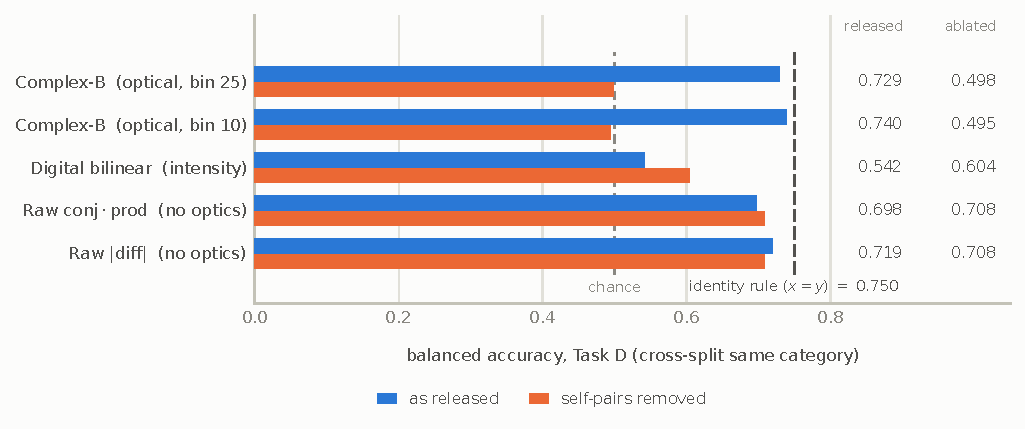
\includegraphics[width=\linewidth]{fig1_taskD_selfpair.pdf}
\caption{\textbf{Task D is accounted for by self-pairs.} Balanced accuracy on
the cross-split same-category task under the refined held-out-category
protocol, before and after removing every self-paired sample $(x,x)$. The
dashed rule at $0.750$ is the accuracy of the measurement-free identity rule
``same category $:=(x=y)$'', which uses the pair labels and no optical data at
all. The optical Complex-B feature does not exceed that rule, and no evidence
of above-chance transfer remains once self-pairs are removed ($0.4979$ at
$\mathrm{bin}=25$ and $0.4948$ at $\mathrm{bin}=10$; point estimates against a
$0.500$ reference, with no significance claimed). The
raw-input baselines, which involve no optical propagation whatsoever, are
unaffected by the ablation.}
\label{fig:D}
\end{figure}

\subsection{Tasks A--C depend on repeat-level splitting}
\label{sec:B3}

Leakage of this kind---correlated repeated measurements of the same unit
distributed across folds---is a documented and widespread failure mode in
machine-learning-based science~\cite{kapoor}, with quantified inflation
reported when the grouping unit is ignored~\cite{rosenblatt}. Throughout this
subsection, ``leakage'' means leakage relative to a claim of out-of-pair or
semantic generalisation. If the tasks were intended only to ask
whether repeated measurements of an already-observed pair can be recognised,
splitting repeats at random is legitimate; the tasks then simply cannot
support claims about category structure or new pairs.

The released scoring applies \code{StratifiedKFold} over 320 samples
comprising 64 pairs $\times$ 5 physical repeats, so repeats of the same pair
are split between training and test folds. We measure the pairwise repeat
correlation of the Complex-B feature directly: mean $0.9828$, with $97.0\%$ of
repeat pairs exceeding $0.97$ (Fig.~\ref{fig:corr}), confirming the authors'
own figure. Training and test folds thus contain near-duplicates of the same
measurement.

Re-scoring with \code{StratifiedGroupKFold} grouped by ordered pair gives
Table~\ref{tab:ABC} and Fig.~\ref{fig:leak}. Pair identity is not evaluable as
an out-of-pair generalisation task when the ordered pair is the grouping unit,
because each 64-way class corresponds to exactly one group. Task C decreases
from $1.0000$ to $0.0474$ under the primary pair-grouped analysis; across the
fold-count sweep the point estimates range from $0.043$ to $0.109$, against a
16-class reference of $0.0625$. We do not interpret these small-sample point
estimates as significantly above or below that reference. We verified that the Task-C collapse is not
an artefact of the fold count: across $n_{\text{splits}}\in\{2,4,5,8\}$ every
test class is represented in training ($100\%$) and accuracy remains in
$0.043$--$0.109$ at both readouts (Fig.~\ref{fig:leak}c).

\begin{figure}[!htbp]
\centering
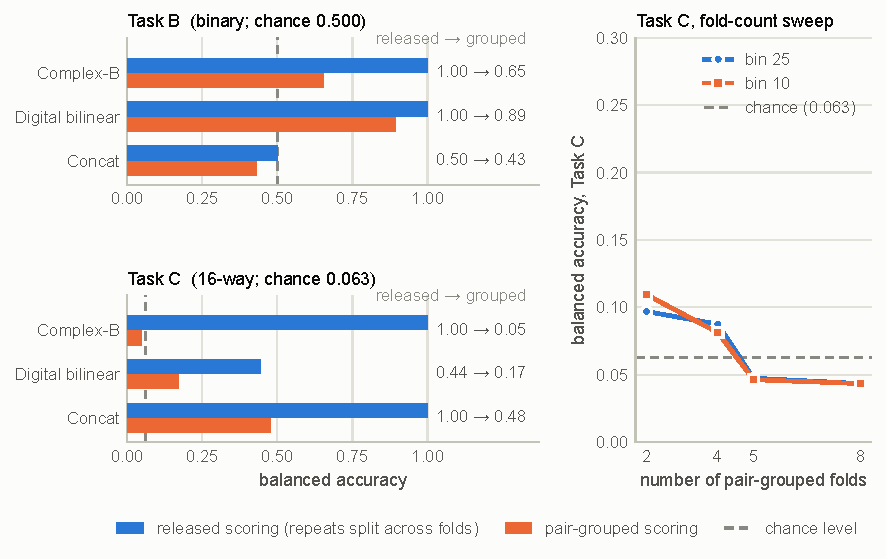
\includegraphics[width=\linewidth]{fig2_leakage.pdf}
\caption{\textbf{Tasks B and C depend on repeat-level splitting.} Left,
balanced accuracy at $\mathrm{bin}=25$ under the released scoring, which
splits the five physical repeats of a pair across folds, and under
pair-grouped scoring, which does not; the value column gives released
$\rightarrow$ grouped for each feature family. Right, the Task-C outcome is
not a fold-count artefact: it persists across
$n_{\text{splits}}\in\{2,4,5,8\}$ at both readouts, with every test class
represented in training in all cases.}
\label{fig:leak}
\end{figure}

\begin{figure}[!htbp]
\centering
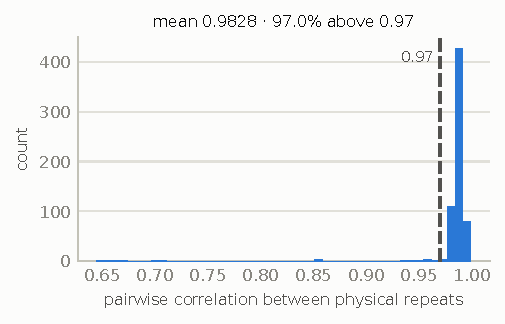
\includegraphics[width=0.68\linewidth]{fig3_repeat_correlation.pdf}
\caption{\textbf{Physical repeats are near-duplicates.} Distribution of
pairwise correlations between the five repeated measurements of the Complex-B
feature, over all 64 ordered pairs at $\mathrm{bin}=25$. Under the released
scoring these near-duplicates are distributed across training and test folds.}
\label{fig:corr}
\end{figure}

\begin{table}[!htbp]
\centering
\caption{Tasks A--C at $\mathrm{bin}=25$, balanced accuracy, released scoring
versus pair-grouped scoring.}
\label{tab:ABC}
\begin{tabular}{llccc}
\toprule
Feature & Task & released & pair-grouped & $\Delta$ \\
\midrule
Complex-B        & A (64-way)  & 1.0000 & \multicolumn{2}{c}{degenerate by construction} \\
Complex-B        & B (binary)  & 1.0000 & 0.6522 & $-0.3478$ \\
Complex-B        & C (16-way)  & 1.0000 & 0.0474 & $-0.9526$ \\
Digital bilinear & B (binary)  & 1.0000 & 0.8917 & $-0.1083$ \\
Digital bilinear & C (16-way)  & 0.4437 & 0.1709 & $-0.2729$ \\
\bottomrule
\end{tabular}
\end{table}

\subsection{The designated Task-B partition is not exceptional}
\label{sec:B4}

Pair-grouped scoring leaves Task B at $0.6522$, above the binary chance level.
This residual admits an exact test, in the label-permutation family
of~\cite{ojala}: because the admissible label assignments can be enumerated,
the permutation null is exact rather than sampled. The same-category label is
fixed entirely by a partition of the eight tokens into four unlabelled
two-token categories,
and there are $8!/((2!)^4 4!) = 105$ such partitions. We therefore recompute
the pair-grouped Task-B accuracy under every admissible assignment. The
designated semantic assignment is a member of this set, so the exact one-sided
$p$-value is the fraction of assignments scoring at least as high as the
designated one, with the designated assignment counted in the numerator; no
Monte Carlo sampling and no continuity correction are involved.

The designated assignment scores $0.6522$ against a null with mean $0.7280$
and standard deviation $0.0347$, and $102$ of the $105$ assignments score at
least as high (Fig.~\ref{fig:perm}); the exact one-sided $p$ is $0.9714$.
Approximately $97\%$ of all admissible category assignments therefore achieve
accuracy at least as high as the designated semantic one. The residual is not
evidence that the measurement recovers the designated category structure.

\begin{figure}[!htbp]
\centering
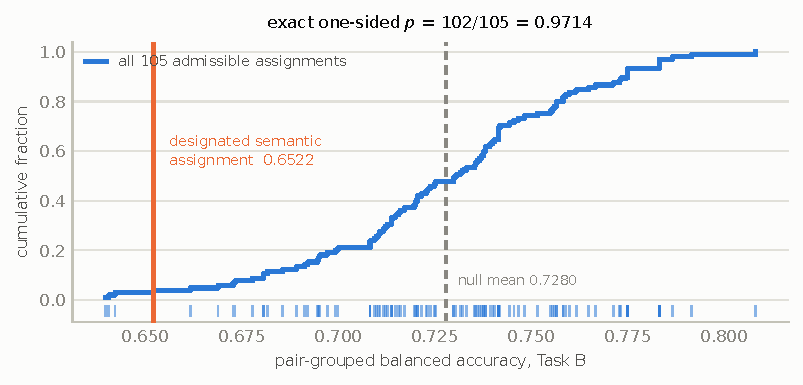
\includegraphics[width=0.80\linewidth]{fig4_permutation_null.pdf}
\caption{\textbf{The residual Task-B accuracy is not exceptional.} Empirical
cumulative distribution and rug plot of pair-grouped Task-B balanced accuracy
over \emph{all} 105 partitions of the eight tokens into four unlabelled
two-token categories---an exact enumeration, not a Monte Carlo sample. The
designated semantic assignment lies in the lower tail.}
\label{fig:perm}
\end{figure}

\subsection{The Task-D shortcut is learned}

Removing self-pairs from the training set and from the test set are distinct
interventions, and crossing them separates a cue that the classifier acquires
during fitting from a structural shortcut sitting in the test set.
Table~\ref{tab:2x2} gives the full design. Above-chance performance occurs
only when self-pairs are present on \emph{both} sides; removing them from
either side leaves no evidence of above-chance transfer. In particular, when
self-pairs are present at test time but absent during training, accuracy is
$0.4917$---the shortcut is available but unused. This is a learned self-pair
shortcut under this evaluation protocol, in the sense of~\cite{geirhos}: a cue
that is predictive within the evaluation as constructed, and that the
classifier adopts in preference to the intended relation. We note the small effective sample: each held-out
fold contributes only 4 distinct positive pairs (2 after ablation) against 24
distinct negatives.

\begin{table}[!htbp]
\centering
\caption{Task D at $\mathrm{bin}=25$ under the full $2\times2$ self-pair
design. Identical classifier, folds and scoring throughout.}
\label{tab:2x2}
\begin{tabular}{llcc}
\toprule
Self-pairs in training & Self-pairs in test & balanced accuracy & test $+$/$-$ \\
\midrule
present & present & 0.7292 & 20 / 120 \\
present & removed & 0.4792 & 10 / 120 \\
removed & present & 0.4917 & 20 / 120 \\
removed & removed & 0.4979 & 10 / 120 \\
\bottomrule
\end{tabular}
\end{table}

\subsection{The XOR evaluation tests repeat recognition}
\label{sec:xor}

The four-token XOR showcase is the second experiment used to support the
computational interpretation of Complex-B, and its logic differs from the
semantic benchmark: an additive linear readout on concatenated single-token
features genuinely cannot express a parity relation, whereas a product feature
can. That identity is not in dispute. What we test is whether the released
evaluation demonstrates a generalisable interaction feature.

The experiment contains all 16 ordered token pairs, each measured five times,
with relation label $y_{\mathrm{XOR}}(x,y)=(x+y)\bmod 2$: eight positive and
eight negative ordered pairs. The relation is symmetric, and all four
self-pairs belong to the negative class. Parity here is a property of the
token \emph{index}; the tokens themselves are random phase patterns generated
from unrelated seeds, so parity is not an encoded optical attribute.

We first reproduce the released sample-level evaluation exactly: Complex-B
attains balanced accuracy $1.0000$ on both 16-way pair identity and binary XOR
classification. That split distributes the repeated measurements of every
ordered pair across training and test folds. Because Complex-B also identifies
the 16 observed pairs perfectly, the XOR score cannot distinguish learning the
parity relation from recognising a pair and recalling its previously observed
label. For a representation that resolves every pair, any fixed pair-to-label
table is learnable; no XOR-specific geometry is required.

We therefore re-evaluate with the physical pair, rather than the camera
repeat, as the unit of generalisation (Fig.~\ref{fig:xor}). Because the number
of distinct pairs is small enough that fold composition matters, we report
both grouped $K$-fold estimates and exhaustive leave-one-group-out, pooling
all out-of-fold predictions before scoring once---per-fold scoring is
undefined here, since a held-out ordered pair contains a single class.
Complex-B gives $0.5000$ (ordered-pair $K$-fold), $0.6250$ (unordered-pair
$K$-fold), $0.5875$ (exhaustive leave-one-ordered-pair-out), $0.3750$
(exhaustive leave-one-unordered-group-out) and $0.4979$ when a token is
excluded from training entirely. We report these as point estimates against a
$0.500$ reference. Their test sets differ in size and in dependence structure,
so we neither pool them nor attach a common uncertainty band, and their
non-monotone ordering should not be interpreted. What they share is that the
released value of $1.0000$ is not retained once repeated observations of the
test pair are excluded from training, and that none of these small-sample
evaluations establishes above-chance transfer.

One grouped value does require explanation. The digital bilinear baseline
reaches $0.8125$ under ordered-pair grouping, above Complex-B. This is a
leakage artefact with an exact mechanism: the feature $z(x)\odot z(y)$ is
algebraically symmetric, so when $(x,y)$ is held out its mirror $(y,x)$
remains in training with a numerically identical feature vector. Removing the
mirror as well collapses it to $0.0625$. Complex-B, whose measured
swap-conjugate correlation is $0.60$ (Sec.~\ref{sec:ideal}), leaks partially
by the same route: $0.5875$ under ordered grouping against $0.3750$ once
mirrors are grouped together.

Two caveats bound these numbers. First, with 16 distinct pairs and 80 samples,
exhaustive leave-one-out is dominated by design artefacts: the concatenation
baseline scores exactly $0.0000$ under both exhaustive regimes, the signature
of anti-learning induced by removing a sample from a balanced design rather
than a meaningful below-chance result. Second, the task admits strong
non-optical structural rules. Because every self-pair is negative, the
measurement-free rule ``negative if $x=y$, positive otherwise'' attains
balanced accuracy $0.7500$; and if each token's parity group is read from its
index, the relation is determined exactly with no optical measurement at all.

Finally, we enumerate all three ways to divide four tokens into two unlabelled
groups of two. Under the same grouped evaluation the designated parity
assignment scores $0.6250$, equal to one alternative and below the remaining
assignment at $0.7125$. With only three admissible assignments this is
descriptive rather than inferential, but it supplies no evidence that the
designated parity structure is preferentially represented.

The mathematical statement that multiplicative features represent XOR where an
additive linear readout cannot is not in dispute, and we do not claim that
Complex-B lacks bilinear information. What the released experiment does not
establish is that the measured field supplies a generalisable XOR interaction
rather than a stable identifier of the 16 observed pairs.

\begin{figure}[!htbp]
\centering
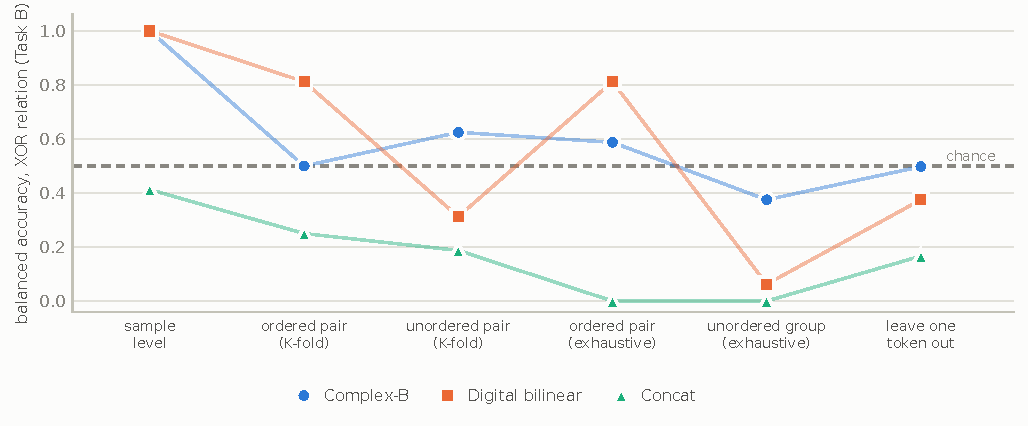
\includegraphics[width=\linewidth]{fig5_xor_splits.pdf}
\caption{\textbf{The XOR result depends on the unit of generalisation.}
Balanced accuracy on the parity relation under six splitting regimes, from the
released sample-level split (repeats of a pair split across folds) to
leave-one-token-out. The regimes are categorical and are deliberately not
joined by lines; markers are offset vertically within each row so that
coincident values remain visible---at sample level both bilinear families sit
at $1.0000$. The digital-bilinear value at exhaustive ordered-pair grouping is
a mirror-pair leakage artefact: $z(x)\odot z(y)$ is symmetric, so the held-out
pair's mirror carries an identical feature vector. Point estimates are shown
against a $0.500$ reference with no uncertainty band, since the regimes differ
in test-set size and dependence structure.}
\label{fig:xor}
\end{figure}

\subsection{The strongest reading available to the original evaluation}
\label{sec:defence}

The findings above are not a claim that the reported accuracies are wrong. We
reproduce every one of them. They are a claim about what those accuracies
establish, and it is worth stating the authors' strongest position explicitly
rather than leaving it to be raised in reply.

That position is that the released tasks were never intended to demonstrate
generalisation to unseen pairs. On this reading, the sample-level split is an
appropriate test of measurement stability and of linear decodability on a
fixed, fully measured pair library; the XOR construction serves to illustrate
the representational capacity of a bilinear feature relative to an additive
linear readout; and the staged reports do qualify the claim, describing the
result as holding ``under the tested evaluation protocol''.

We accept that reading, and under it the released numbers stand. Our point is
what follows from it. A sample-level evaluation over a fixed pair library
cannot separate three distinct hypotheses: that the feature encodes the
relation, that it encodes pair identity from which a memorised label table is
recovered, or that it exploits a structural cue such as the self-pair
alignment. Because Task A shows that Complex-B resolves all 16---and all
64---observed pairs perfectly, the second hypothesis alone suffices to produce
the reported relation accuracies, and no relation-specific structure in the
measurement is required. The evidence is therefore consistent with the
measurement being informative about the observed pairs, and does not
discriminate among the mechanisms that could produce that.

This matters because the manuscript's interpretation does not stay at the
level of observed-pair decodability. Claims about semantic relational
structure, about pairwise relational computation, and about analogy to
attention are all claims about a relation that transfers. That transfer is
what the released evaluations do not test.

\section{Computational interpretation}
\label{sec:operator}

Equation~\eqref{eq:B} is the cross term of two-beam interference, isolated by
four-step phase shifting. Under linear optics the jointly demodulated field
and the digital product $A_x^{\ast}\!\odot A_y$ of the separately measured
complex output fields $A_x, A_y$ are the same quantity up to noise. The
decisive control is therefore an equality test between the jointly demodulated
field and that digital product, formed from the fields the \emph{actual} two
arms produce. We deliberately do not phrase this as a shared-$T$ test: as
Sec.~\ref{sec:ideal} shows, the released estimator does not closely satisfy
the shared-operator identities, so $A_x=T_xE_x$ and $A_y=T_yE_y$ with
$T_x\neq T_y$ must be admitted. The shared-operator case is a special
instance, not the general requirement.

The released controls are not this test. The ``digital bilinear'' baseline is
$z(x)\,z(y)$ where $z$ is binned camera \emph{intensity}, discarding phase;
a further variant is described in the supplement as a per-channel product
``no cross-conjugation''; and the pseudo-$B$ control replaces the physical $T$
with a random complex Gaussian. The first two compare different algebraic
objects; the third asks whether a real scattering matrix differs from a random
one, not whether joint measurement yields information unavailable to separate
measurement. The required control is absent, and---because this experiment
records only single-token \emph{intensity}---it cannot be performed on the
released data. It can, however, be performed on the same apparatus: the
self-referenced transmission-matrix measurement in the earlier studies of the
same work recovers exactly the complex fields it requires.

\subsection{Relation to established optical technique}
\label{sec:priorart}

This section is a scoped bibliographic comparison based on the principal
methods and claims associated with these works; it is not an exhaustive,
apparatus-level priority analysis. Each work below is cited for its headline
contribution only, and we attach no finer device correspondence to any of
them.

Two questions are worth separating, because the manuscript's abstract and its
own staged reports answer them differently: whether the demodulation is new,
and whether the use to which it is put is new.

On the first, the technique is established. Recovering an interference term
from a small set of intensity frames taken at stepped reference phases is the
basis of phase-shifting interferometry~\cite{bruning}, and recovering a full
complex field from intensity-only measurements by the same route is
standard~\cite{yamaguchi}. This is consistent with the authors' own
characterisation of phase-stepping interferometry as a mature technique.
The potentially distinctive element is therefore not the demodulation identity
itself, but the particular combination of two encoded inputs, a fixed
scattering transformation, channel-resolved recovery, and the interpretation
of the result as a computational feature. Our search was not exhaustive and
does not establish whether that combination is unprecedented.

On the second, each ingredient has substantial precedent in optical computing.
Recovering complex per-channel quantities through a random scattering operator
by phase stepping is how transmission matrices are
measured~\cite{popoff}. Obtaining a product of two encoded optical fields by
square-law detection is an established route to optical
multiplication~\cite{hamerly}. Using a fixed scattering medium as a random
feature map is the basis of optical reservoir computing~\cite{rafayelyan}.
Optical convolution and correlation of two inputs have been established since
the 1960s~\cite{vanderlugt,weaver}; we cite these as evidence that the general
practice is long-standing, not as evidence of equivalence to the present
apparatus, whose operator, output representation and purpose differ.
Establishing physical novelty therefore requires identifying which property of
the combination was absent from prior optical correlators, scattering-based
processors and coherent multiplication architectures---a determination the
released materials do not make, and one that a systematic full-text prior-art
review would be needed to settle. We record the position as \emph{novelty not
established}, which is distinct from novelty absent.

\subsection{What is, and is not, implemented relative to attention}
\label{sec:attention}

The manuscript describes the measured quantity as structurally analogous to a
core operation in Transformer attention. We set out precisely how far that
correspondence extends, because the claim is otherwise easy to read as
stronger than the experiment supports.

An attention compatibility score~\cite{attention} is
\begin{equation}
  s(x,y) \;=\; x^{\top} W_Q^{\top} W_K\, y ,
\end{equation}
while a measured detector channel supplies
\begin{equation}
  B_k(x,y) \;=\; x^{\dagger} K_k\, y .
\end{equation}
Both are two-input bilinear (respectively sesquilinear) compatibility forms,
so the stated analogy holds in that weak mathematical sense, and we do not
dispute it at that level.

The differences are the substance. $W_Q$ and $W_K$ are learned, may be
distinct, and their product is a general matrix; $K_k$ is fixed by the medium
during the reported experiment and is not learned end-to-end. Under the ideal shared-operator model each
unbinned $K_p$ is a rank-one positive semidefinite outer product and a binned
$K_k$ is a finite sum of such terms, so the realisable operator family is a
restricted subclass rather than a general learnable bilinear map---though, as
Sec.~\ref{sec:ideal} notes, if the two arms do not share an operator this
particular restriction is weaker than it appears. Beyond the operator itself,
the experiment does not construct a token-pair score matrix, and it implements
no scaling, no softmax normalisation, no masking, no value projection and no
value aggregation. No end-to-end attention task is run, and the readout is a
linear classifier applied digitally to the measured features.

The defensible reading is therefore that the experiment demonstrates a
restricted physical pair-feature primitive, not an implementation of
Transformer attention and not attention hardware. Proposed photonic
self-attention architectures supply the relevant category
distinction~\cite{lightening}: implementing a bilinear primitive is not the
same as implementing an attention layer, which ordinarily requires
programmable projections, formation of a score structure, normalisation or an
explicit substitute for it, and value-side processing. We cite that work as an
architecture proposal, not as measured hardware, and we do not enter such
systems as comparanda, since a like-for-like comparison would require
throughput and energy figures the released analysis does not report.

\subsection{Scale, effective dimensionality, and unmeasured outlooks}

\paragraph{Scale and effective dimensionality.}
The released computational demonstration contains eight fixed tokens and
64 ordered pairs, all derived from one deterministic random-phase codebook.
It therefore does not test generalisation to a larger vocabulary, to newly
encoded tokens, to another random codebook, or to an independently acquired
physical operator. The Result-4 study itself identifies vocabulary scale as a
limitation and notes, in the authors' released Report 4, that a related
token-family representation previously exhibited degeneracy-boundary collapse
at $N=16$.

Nominal detector dimensionality should also be distinguished from effective
dimensionality on the evaluated data. At the main-text bin size of 25 pixels,
we reproduce a participation-ratio effective rank of 3.00 for the released
Complex-B feature ensemble, despite hundreds of nominal detector channels;
at bin size 10 the corresponding value is 9.62. These quantities are
properties of the observed eight-token feature ensemble, not universal rank
bounds on the apparatus. They nevertheless show that the high-dimensional
capacity invoked in the computational interpretation was not demonstrated on
the benchmark used to support it: most observed variation is concentrated in
a small number of effective complex directions, and near-saturated accuracy
is obtained on a correspondingly small, repeatedly observed vocabulary.

\paragraph{Speed and energy are unmeasured outlooks.}
The experiment establishes that the complex cross term can be recovered on
the physical platform; it does not establish a system-level speed or energy
advantage. In the released acquisition protocol, each ordered input pair is
measured through four sequential phase settings. The overall protocol also
contains blank-control measurements, camera readout, calibration,
normalisation, demodulation, and digital classification. Blank controls may
be reused across multiple pairs and therefore should not automatically be
counted as a per-pair cost, but they remain part of the demonstrated system.

No end-to-end latency, pair-score throughput, energy per recovered score,
total system power, or amortised calibration cost is reported in the public
materials. Nor is the demonstrated implementation compared under a matched
accuracy and precision target with a GPU, FPGA, or digital complex
correlator. The current experiment acquires the ordered pairs individually;
it does not demonstrate parallel construction of an $N\times N$ score
matrix, softmax normalisation, value projection, or value aggregation.
Future spatial, wavelength, or temporal parallelisation may change this
assessment, but it is not measured here. Statements concerning high-speed or
energy-efficient Transformer-like hardware should therefore be read as
prospective motivation rather than experimental findings of the present
study.

\section{Discovery attribution and protocol status}
\label{sec:provenance}

The central claim is causal: that an agent, rather than its training
distribution or its operators, originated the mechanism. Searching the full
deposit we find no backbone model name or version, no system or initial
prompts, no agent trace, no record of human intervention, and no
direction-selection log; the deposit states explicitly that the engine and
hardware-control software are not included. What is released---result-level
data and offline analysis scripts---establishes that the numbers can be
recomputed. It cannot establish where the idea came from.

We note a further tension internal to the released material. The staged
reports characterise the contribution in measured terms: phase-stepping
interferometry is ``a mature technique'', and ``the methodological novelty is
not the demodulation itself but its application to extract a computationally
meaningful bilinear observable''. The abstract of the manuscript describes the
same object as a ``previously unreported physical mechanism''. We record this
as an internal inconsistency in how the contribution is characterised. It is
not a completed novelty audit; Sec.~\ref{sec:priorart} sets out how far the
established literature reaches and what a determination would still require.
Our position is that physical novelty is \emph{not established} by the
released materials, not that it is absent.

\subsection{Architectural attribution}

A separate attribution problem sits beneath the provenance one, and survives
even if the trajectory were accepted as fully autonomous. The audited preprint
credits specific components of its agent system---the ones it names Meta-Trace,
the dual-layer separation, role--phase decoupling and accumulated research
experience---with sustaining the long-horizon trajectory. A single successful run cannot
identify which component, if any, produced the outcome. The released material
contains no single-agent baseline, no run with Meta-Trace replaced by ordinary
rolling summarisation, no fixed-workflow comparison, no ablation of the
Critical Reviewer role, no run without inherited prior-study experience, no
variation of random seed, and no variation of backbone model. Nor is there a
human-expert time or cost baseline against which the reported speed advantage
could be assessed. The reported totals---145.9 million tokens, 3{,}242 model
calls, 1{,}242 tool invocations---are resource counts. They record what was
spent, not which architectural choice was responsible for what was obtained.

\subsection{Evaluation search space}
\label{sec:search}

The evaluation supporting the computational claim involves several free
choices, and the released material shows that more than one value of most of
them was examined. Table~\ref{tab:search} records the search space that is
publicly visible, alongside what the public record does and does not establish
about when each choice was fixed. We stress the distinction: for none of these
choices do the released materials document the selection \emph{timing}, and we
therefore do not assert that any of them was made after inspecting the
outcome. What the record does establish is that the reported configuration was
selected from a searched space without an independent confirmation set. This
is adaptive evaluation, and the standard remedy---pre-registration of the
readout parameters and splits, or a held-out physical realisation on which the
selected configuration is evaluated once---was not applied. The distinction
being drawn is the exploratory/confirmatory one, and pre-registration is the
instrument that makes it inspectable rather than a matter of
assertion~\cite{nosek}.

\begin{table}[!htbp]
\centering\small
\caption{Publicly visible evaluation search space for the Result-4 benchmark.}
\label{tab:search}
\setlength{\tabcolsep}{4pt}
\begin{tabular}{L{3.2cm}L{4.2cm}L{3.6cm}L{2.9cm}}
\toprule
Choice & Publicly observed search & Selection timing & Independent confirmation \\
\midrule
Detector bin & 5, 10, 25 & Not publicly documented & None identified \\
Output budget & multiple $n_{\text{out}}$ values & Not publicly documented & None identified \\
Task-D protocol & multiple descriptions and implementations & Protocol evolution observed & None identified \\
Feature family & multiple optical and digital families & Exploratory analysis evident & None identified \\
Token vocabulary & one fixed random codebook & Not publicly documented & No independent vocabulary \\
\bottomrule
\end{tabular}
\end{table}

\paragraph{Protocol evolution and confirmatory status.}
The released reports document an evolving analysis rather than one fixed
confirmatory protocol. Report 4 and Report 5 describe different
cross-split constructions and report materially different behaviour across
feature families. The later analysis additionally explores detector bin
sizes, output-channel budgets, sparse-tap selections, raw-input controls,
random-operator controls, and revised task definitions. Such exploration is
scientifically useful and, when reported transparently, is not itself an
error. Because the documented Task-D protocols are not identical, we do not
treat numerical differences between the two reports as controlled
method-to-method comparisons.

It does, however, change the evidential status of the resulting performance
comparisons. The public materials do not document when the token vocabulary,
task definitions, split rules, bin size, output budget, or highlighted
operating point were fixed relative to inspection of the corresponding
outcomes. No independently acquired confirmation set or new physical
operator is used after these choices. We therefore interpret the released
performance landscape as exploratory. A confirmatory computational claim
would require a frozen protocol evaluated on new tokens, a new codebook, an
independent acquisition, or another physical realisation without further
selection of readout configuration.

\section{Limitations and evidence needed}
\label{sec:settle}

Before setting out what further evidence would help, we separate three things
that this paper has deliberately kept apart, because reading them as one
category would misstate our result.

\emph{Direct findings of this audit}, each established by an ablation or an
exact test on the released data: the mismatch between the evaluation unit and
the claimed unit of generalisation; the fact that the designated category
assignment is not exceptional among all 105 admissible assignments; the
self-pair shortcut in Task D; and the mirror-pair reuse in the XOR showcase.

\emph{Absences in the public record}, which are not findings about the
underlying work: no operator-matched digital reconstruction, no
backbone-model or prompt disclosure, no agent trace or intervention log, no
architectural ablation, and no documentation of when the readout and split
choices were fixed.

\emph{Outside our scope}, on which we take no position: the transmission-matrix
reproduction and the majorization-order study; the hardware performance of the
platform; and an exhaustive priority determination for the measurement
mechanism.

Our findings identify a failure of evidential attribution, not a failure to
produce repeatable optical measurements. The released experiments show that
the platform yields stable and decodable pair-dependent signals. They do not
yet determine whether the decoded structure is relation-specific, whether the
optical stage improves on an operator-matched digital reconstruction, or
permit the origin of the scientific interpretation to be distinguished among
model prior knowledge, agent-level synthesis and human steering.

These evidential limitations are addressable. They require different evidence for the
computational, physical, and autonomy claims; no single additional accuracy
value would address all three.

\paragraph{Agent provenance.}
Attribution of an idea to an autonomous agent requires disclosure of the
backbone model and exact version, inference settings, initial and system
prompts, retrieval sources, progressively disclosed skills, candidate
directions, direction-selection decisions, and human interventions. The
complete time-ordered Meta-Trace and tool trajectory should be released in a
form that distinguishes contemporaneous records from summaries produced
after the experiment. If safety, licensing, or instrument-access constraints
prevent release of particular implementation details, the omitted fields and
their relevance to the claimed discovery should be identified explicitly.
Result-level data alone cannot establish the causal origin of the hypothesis.

\paragraph{Prior-availability control.}
The relevant question is not whether a current language model can reproduce
the mechanism after publication, but whether the backbone available to the
agent before the study already contained or could readily elicit the same
proposal. This should be tested using the exact original model snapshot,
without the agent scaffold or experimental feedback, from the same initial
platform description. The prompt, decoding parameters, number of independent
queries, retrieval permissions, and a prospectively defined scoring rule
should be fixed before inspection of the outputs. The assessment should
separately record whether the model proposes the interference cross term and
whether it identifies the underlying phase-stepping and coherent-detection
principles as established knowledge. Such a control would measure prior
availability; it would not by itself prove the causal origin of the observed
trajectory.

\paragraph{Operator-matched physical control.}
For each detector pixel, the ideal shared-operator model predicts
\begin{equation}
 B_p(x,y)=(TE_x)_p^{*}(TE_y)_p .
\end{equation}
For a binned channel $\mathcal{B}_k$, the corresponding reconstruction is
\begin{equation}
 \bar B_k^{\mathrm{digital}}(x,y)
 =
 \sum_{p\in\mathcal{B}_k}
 (TE_x)_p^{*}(TE_y)_p .
\end{equation}
The decisive control is therefore to measure the two propagated complex
fields separately under the same physical operator and compare this digital
reconstruction, channel by channel, with the jointly demodulated
$\bar B_k^{\mathrm{physical}}$. Agreement should be quantified in amplitude,
phase, residual structure, repeatability, and downstream performance under
identical feature budgets and splits. If the two input arms implement
different operators, the corresponding $T_x^{\dagger}T_y$ model should be
stated and tested instead. This experiment would determine whether joint
measurement supplies information beyond separately measured complex fields;
intensity products and random-operator pseudo-$B$ controls do not answer that
question.

\paragraph{Benchmark with a valid unit of generalisation.}
A confirmatory benchmark should contain relational structure in the inputs
rather than attach semantic labels to independent random vectors. It should
use tokens, codebooks, or physical inputs not involved in configuration
selection. All repeated measurements of the same physical condition must
remain in the same fold whenever the claim concerns generalisation to new
conditions. Self-pairs should either be excluded from relation evaluation or
reported as a separate stratum, and performance should be compared with
measurement-free structural rules and an exact or permutation null over
admissible label assignments. Pair identity may be evaluated as repeat
recognition, but it should not be interpreted as out-of-pair generalisation.
The final test should use a new acquisition session, codebook, vocabulary, or
physical operator after the evaluation protocol has been frozen.

\paragraph{Independent agent and hardware replications.}
A single successful trajectory cannot establish that the reported outcome is
a reproducible property of the agent architecture. The open-ended study
should be repeated independently from the same initial information, with all
runs and unsuccessful directions retained. At least three complete runs would
provide a minimal existence check, although more are required to estimate a
meaningful discovery rate for a stochastic system. Replication should also
separate agent stochasticity from hardware specificity by including, where
feasible, an independent acquisition session or physical realisation. The
reported outcomes should include the frequency with which the mechanism is
proposed, selected, experimentally supported, rejected, or replaced by
another direction.

\paragraph{Pre-registered confirmation.}
Before the confirmatory run, the token set, task definitions, train--test
unit, treatment of self-pairs, detector binning, output budget, feature
families, classifier, hyperparameters, primary endpoint, and statistical
comparison should be frozen in a time-stamped protocol. Exploratory searches
over bin size, $n_{\mathrm{out}}$, task construction, or feature family may be
reported in full, but the selected configuration should then be evaluated on
untouched data without further adaptation. This separation would turn the
released performance landscape from an exploratory result into a test of a
specified computational claim.

Together, these additions would not require treating autonomous discovery as
a binary label. They would allow readers to distinguish four progressively
stronger conclusions: automated execution of a known protocol, recombination
of available scientific knowledge, generation and testing of a new
engineering interpretation, and experimental identification of a finding
not available to the model or its operators beforehand.


\appendix

\section{Model--measurement consistency}
\label{sec:ideal}\label{app:ideal}

This section is diagnostic rather than evaluative. It bears on neither the
benchmark findings of Sec.~\ref{sec:benchmark} nor the central attribution
question, and we report it because it constrains what the released estimator
can be assumed to satisfy.

Under the stated linear-optical model the unbinned channel kernel
$K_p = T_p^{\dagger}T_p$ is \emph{algebraically} rank-one, Hermitian and
positive semidefinite; spatial binning forms $K_k=\sum_{p\in\mathcal{B}_k}K_p$,
a positive semidefinite sum whose algebraic rank is bounded by the number of
independent propagation rows in the bin. These are consequences of the model,
not empirical assumptions, and they imply $B_p(y,x)=B_p(x,y)^{\ast}$.

What the release contains is an estimator carrying a reference arm, phase
stepping, blank subtraction, drift and calibration error. It satisfies the
ideal identities only approximately. Over the 28 off-diagonal token pairs the
mean correlation between $\widehat B(y,x)$ and $\overline{\widehat B(x,y)}$ is
$0.6042$, against $0.1537$ for the uncorrelated comparison $\widehat B(x,y)$;
the conjugate symmetry is thus clearly present but far from exact. On
self-pairs, where the model predicts a positive real value, the real part is
non-negative in every channel, but the mean relative imaginary magnitude
$|\mathrm{Im}\,\widehat B|/|\widehat B|$ is $0.3511$.

A phase-gauge offset would reproduce this signature without implying that the
cross term was not isolated, so we tested it: estimating a single global phase,
and then a per-channel phase, from the self-pairs alone and applying it to all
pairs. Neither accounts for the departure. The self-pair imaginary ratio falls
only from $0.3511$ to $0.3102$ (global) and $0.3057$ (per-channel), and the
swap-conjugate correlation does not improve ($0.5666$ and $0.5606$). The
per-channel phases are moreover nearly identical (circular spread $0.0019$), so
there is no channel-dependent phase structure to remove.

We draw no conclusion about the cause. Two candidate explanations remain open
and are not separable from the released data: a residual in the blank or
reference subtraction, and the two input arms not sharing a transmission
operator, $T_x \neq T_y$. We flag that the second would also weaken one line
of criticism available against the attention analogy, since a kernel
$T_x^{\dagger}T_y$ is rank-one but neither Hermitian nor positive
semidefinite, and is in that respect \emph{less} constrained than the
shared-operator case. Resolving this requires acquisition-level information
that the deposit does not contain.

\section{The PROBE checklist in full}
\label{app:probe}

\paragraph{P --- Provenance disclosure.}
The backbone model and version, its training cut-off relative to the
publication dates of all target papers, the complete initial prompt, every
candidate direction generated and discarded, the criterion by which a
direction was selected and by whom, every human intervention, and the full
agent trace. Without these, the causal attribution ``the agent discovered
$X$'' is not merely unverified but unformulated.

\paragraph{R --- Replication.}
At least three independent runs from the same starting prompt, with the
distribution of outcomes reported. A single trajectory from a stochastic
system cannot distinguish an architectural property from a sampling event.

\paragraph{O --- Operator-matched control.}
Where a physical measurement is claimed to produce information, the control
must be the digital reconstruction of the \emph{same} quantity under the
\emph{same} operator, not a different quantity. Randomising the operator, or
substituting an algebraically distinct expression, tests a different
hypothesis.

\paragraph{B --- Benchmark integrity.}
The evaluation must possess the structure it purports to measure; train/test
partitions must respect the unit of generalisation; and every reported
accuracy must be compared against the best measurement-free rule available on
the same partition, and against an exact or permutation null over the
admissible label assignments where one can be enumerated.

\paragraph{E --- Evaluation pre-registration.}
Readout parameters, feature budgets and splits must be fixed before the
comparison of interest, or the search over them must be reported in full.

\section*{Data and code availability}
All analysis code and result files are at
\url{https://github.com/SII-WANGZJ/Nullius}, with package versions pinned. The
audit generated no data of its own: it consumes only the authors' public
deposit (DOI 10.5281/zenodo.19890402), which is not redistributed here. The
repository records a checksum for every file read from that deposit, so any
subsequent change to it is detectable.

\begin{thebibliography}{99}\small
\bibitem{boiko} D.~A.~Boiko, R.~MacKnight, B.~Kline and G.~Gomes,
  \emph{Autonomous chemical research with large language models},
  Nature \textbf{624}, 570--578 (2023). \doi{10.1038/s41586-023-06792-0}.
  % supports: agents credited with running research, not just assisting.
\bibitem{burger} B.~Burger \emph{et al.},
  \emph{A mobile robotic chemist}, Nature \textbf{583}, 237--241 (2020). \doi{10.1038/s41586-020-2442-2}.
  % supports: autonomous experimentation on real apparatus predates LLM agents.
\bibitem{swanson} K.~Swanson, W.~Wu, N.~L.~Bulaong, J.~E.~Pak and J.~Zou,
  \emph{The Virtual Lab of AI agents designs new SARS-CoV-2 nanobodies},
  Nature \textbf{646}, 716--723 (2025). \doi{10.1038/s41586-025-09442-9}.
  % supports: multi-agent design followed by experimental validation.
\bibitem{qiushi} S.~Yang \emph{et al.},
  \emph{End-to-end autonomous scientific discovery on a real optical
  platform}, preprint (2026). \arxivid{2604.27092}.
\bibitem{zenodo} S.~Yang, \emph{Source materials for
  ``End-to-end autonomous scientific discovery on a real optical platform''},
  Zenodo (2026). \doi{10.5281/zenodo.19890402}.
\bibitem{kapoor} S.~Kapoor and A.~Narayanan,
  \emph{Leakage and the reproducibility crisis in machine-learning-based
  science}, Patterns \textbf{4}, 100804 (2023). \doi{10.1016/j.patter.2023.100804}.
  % supports: leakage as a documented, cross-disciplinary failure mode;
  % motivates auditing split logic rather than headline accuracy.
\bibitem{rosenblatt} M.~Rosenblatt \emph{et al.},
  \emph{Data leakage inflates prediction performance in connectome-based
  machine learning models}, Nat.\ Commun.\ \textbf{15}, 1829 (2024). \doi{10.1038/s41467-024-46150-w}.
  % supports: quantified inflation when correlated repeats cross folds.
\bibitem{ojala} M.~Ojala and G.~C.~Garriga,
  \emph{Permutation tests for studying classifier performance},
  J.\ Mach.\ Learn.\ Res.\ \textbf{11}, 1833--1863 (2010). \href{https://www.jmlr.org/papers/v11/ojala10a.html}{jmlr.org/papers/v11/ojala10a}.
  % supports: the label-permutation null of Sec. B4; the exact enumeration
  % is the finite-population form of their label-permutation test.
\bibitem{geirhos} R.~Geirhos \emph{et al.},
  \emph{Shortcut learning in deep neural networks},
  Nat.\ Mach.\ Intell.\ \textbf{2}, 665--673 (2020). \doi{10.1038/s42256-020-00257-z}.
  % supports: self-pair cue and mirror reuse as shortcuts; the distinction
  % between intended and exploited structure.
\bibitem{bruning} J.~H.~Bruning \emph{et al.},
  \emph{Digital wavefront measuring interferometer for testing optical
  surfaces and lenses}, Appl.\ Opt.\ \textbf{13}, 2693--2703 (1974). \doi{10.1364/AO.13.002693}.
  % supports: stepped reference phase + per-detector intensity -> interference
  % term, as an established measurement principle.
\bibitem{yamaguchi} I.~Yamaguchi and T.~Zhang,
  \emph{Phase-shifting digital holography}, Opt.\ Lett.\ \textbf{22},
  1268--1270 (1997). \doi{10.1364/OL.22.001268}.
  % supports: recovery of a complex field from intensity-only frames.
\bibitem{popoff} S.~M.~Popoff \emph{et al.},
  \emph{Measuring the transmission matrix in optics}, Phys.\ Rev.\ Lett.\
  \textbf{104}, 100601 (2010). \doi{10.1103/PhysRevLett.104.100601}.
\bibitem{hamerly} R.~Hamerly \emph{et al.},
  \emph{Large-scale optical neural networks based on photoelectric
  multiplication}, Phys.\ Rev.\ X \textbf{9}, 021032 (2019). \doi{10.1103/PhysRevX.9.021032}.
  % supports: square-law detection as an established route to optical
  % inner products, relevant to the novelty question.
\bibitem{rafayelyan} M.~Rafayelyan \emph{et al.},
  \emph{Large-scale optical reservoir computing for spatiotemporal chaotic
  systems prediction}, Phys.\ Rev.\ X \textbf{10}, 041037 (2020). \doi{10.1103/PhysRevX.10.041037}.
  % supports: a fixed scattering medium as a random feature map.
\bibitem{vanderlugt} A.~Vander~Lugt,
  \emph{Signal detection by complex spatial filtering}, IEEE Trans.\ Inf.\
  Theory \textbf{10}, 139--145 (1964). \doi{10.1109/TIT.1964.1053650}.
  % supports (headline only): optical correlation as long-established
  % practice. NOT cited for any device-level correspondence.
\bibitem{weaver} C.~S.~Weaver and J.~W.~Goodman,
  \emph{A technique for optically convolving two functions}, Appl.\ Opt.\
  \textbf{5}, 1248--1249 (1966). \doi{10.1364/AO.5.001248}.
  % supports (headline only): optical convolution of two inputs. NOT cited for
  % the form of the recovered term; that would need full-text verification.
\bibitem{attention} A.~Vaswani \emph{et al.},
  \emph{Attention is all you need}, NeurIPS \textbf{30} (2017). \arxivid{1706.03762}.
\bibitem{lightening} H.~Zhu \emph{et al.},
  \emph{Lightening-Transformer: a dynamically-operated, optically
  interconnected photonic transformer accelerator}, in Proc.\ IEEE Int.\ Symp.\
  High-Performance Computer Architecture (HPCA), 686--703 (2024). \doi{10.1109/HPCA57654.2024.00059}.
  % supports: what a full attention layer requires. An accelerator proposal
  % evaluated in simulation, not a fabricated and measured photonic
  % Transformer chip; no performance figure of theirs is used here.
\bibitem{nosek} B.~A.~Nosek, C.~R.~Ebersole, A.~C.~DeHaven and D.~T.~Mellor,
  \emph{The preregistration revolution}, Proc.\ Natl.\ Acad.\ Sci.\ USA
  \textbf{115}, 2600--2606 (2018). \doi{10.1073/pnas.1708274114}.
  % supports: the exploratory/confirmatory distinction and pre-registration as
  % the instrument that makes it inspectable.
\end{thebibliography}

\end{document}
